\documentclass[a4paper, 10pt]{article}
\usepackage[UTF8]{ctex}
\usepackage{geometry}
\usepackage{graphicx}
\usepackage{setspace}
\usepackage{float}
\usepackage{listings}
\usepackage{xcolor}
\usepackage{multirow}
\lstset{
    numbers=left, 
    numberstyle= \tiny, 
    keywordstyle= \color{ blue!70},
    commentstyle= \color{red!50!green!50!blue!50}, 
    frame=shadowbox, % 阴影效果
    rulesepcolor= \color{ red!20!green!20!blue!20} ,
    escapeinside=``, % 英文分号中可写入中文
    xleftmargin=2em,xrightmargin=2em, aboveskip=1em,
    framexleftmargin=2em
} 
\geometry{left = 1.0 cm, right = 1.0cm, top = 2.0cm, bottom = 2.0cm	}
\title{编译原理第五章(三)}
\author{李鹏辉}

\begin{document}
\maketitle 

1.(5.4.4):为下面的产生式写出一个和例5.19类似的L属性SDD。这里的每一个产生式表示一个常见的C语言中那样的控制流结构。你可能需要生成一个三地址语句来跳转到某个标号L,此时你可以生成语句goto L.

1) $S\rightarrow if \;(C)\;S_1 \; else \; S_2$

2) $S\rightarrow do \; S_1 \; while\; (C)$

3) $S\rightarrow '\{'  \;L \;'\}' \;; L \rightarrow LS \;| \;\varepsilon$

请注意,列表中的任何简单语句都可能包含一条从它内部跳转到下一条语句的跳转指令,因此简单地每个语句按顺序生成代码是不够的。

1)

$L_1 = new()$

$L_2 = new()$

$L_3 = new()$

$S_1.next = S.next$

$S_2.next = S.next$

$C.false = L_2$

$C.true = L_1$

$S.code = C.code||label||L_1 ||S_1.code||goto\;\; L_3 || label || L_2 || S_2.code || lable || L_3$


2)

$L_1 = new()$

$L_2 = new()$

$C.true = L_1$

$C.false = S.next$

$S_1.next = L_2$

$S.code =  label||L_1 || S1.code ||lable||L_2|| C.code$

3)

$S.code = L.code$

$L.code = L_1.code || S.code$


2.(5.5.4)按照5.3.3的风格,将5.4.4中得到的每个SDD和一个LL语法分析器一起实现,但是代码风格(或指向代码的指针)存放在栈中

1. 
\begin{figure}[H]
\centering
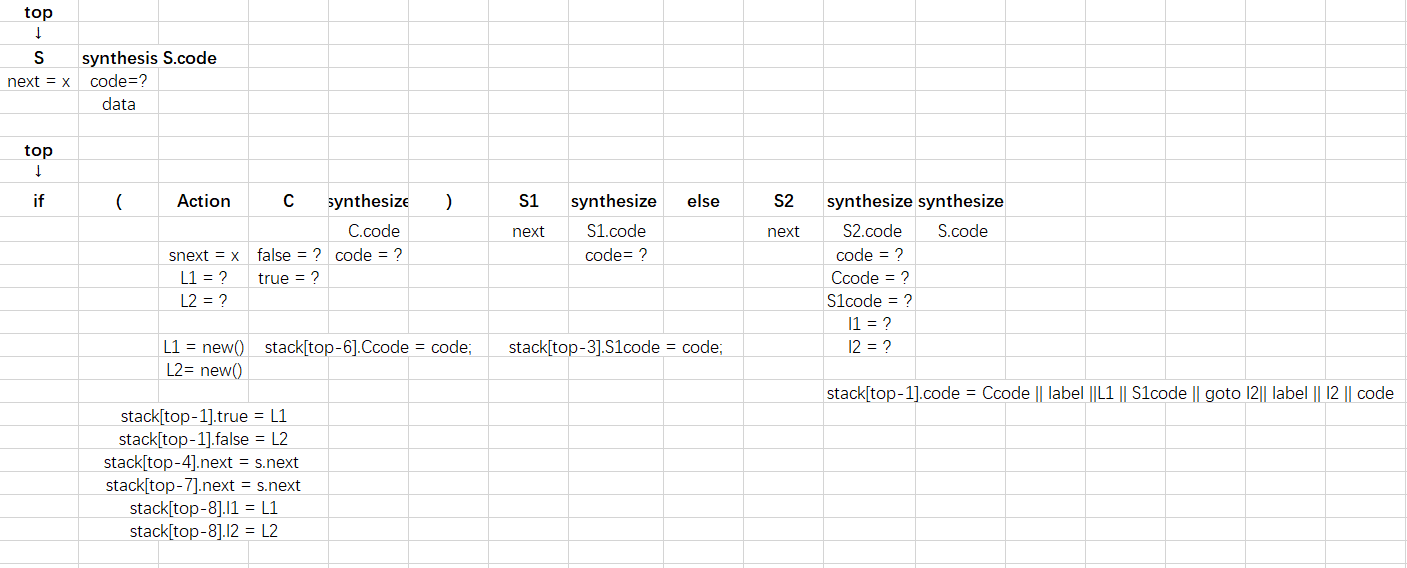
\includegraphics[scale=0.6]{chapter5_hw3_1}
\end{figure}

2. 
\begin{figure}[H]
\centering
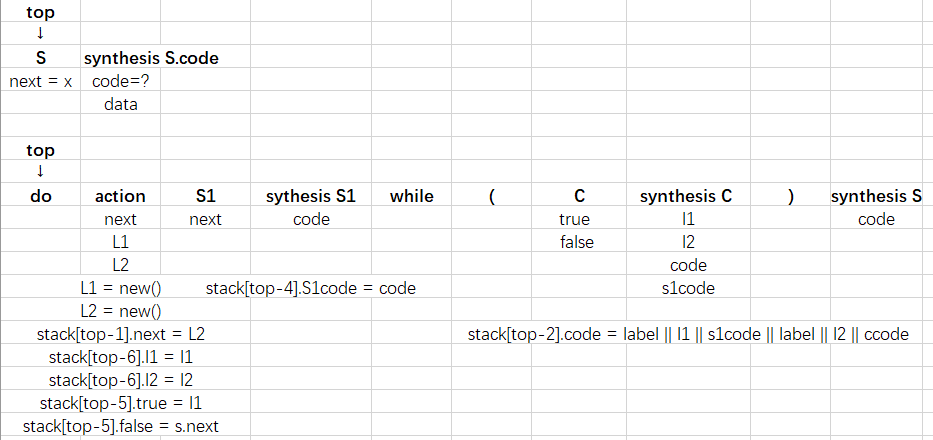
\includegraphics[scale=0.6]{chapter5_hw3_2}
\end{figure}


3. 消除左递归后得到

$S \rightarrow '\{' L  '\}'$

$L \rightarrow L'$

$L' \rightarrow SL' | \varepsilon$

\begin{figure}[H]
\centering
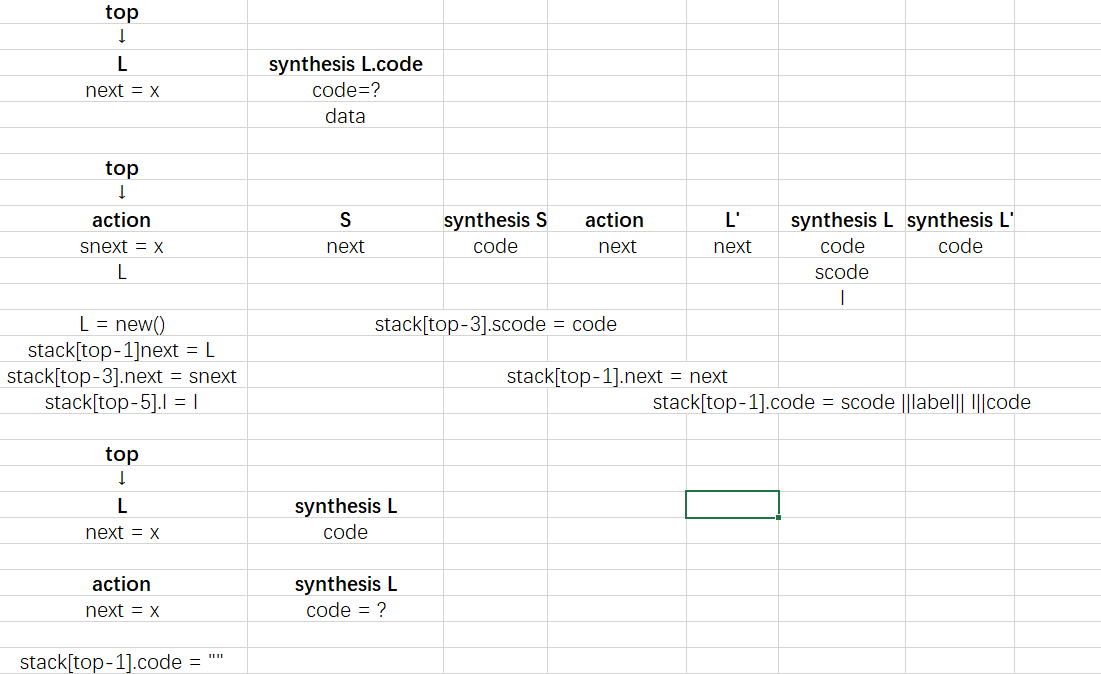
\includegraphics[scale=0.6]{chapter5_hw3_3}
\end{figure}


3.(5.5.5)按照5.5.4的风格,将5.4.4中得到的每个SDD和一个LR语法分析器一起实现

5.5.4和5.5.5写出翻译方案即可,注意5.5.4的动作位置,而5.5.5参照5.5.4节,把规约动作放在最右端

\begin{figure}[H]
\centering
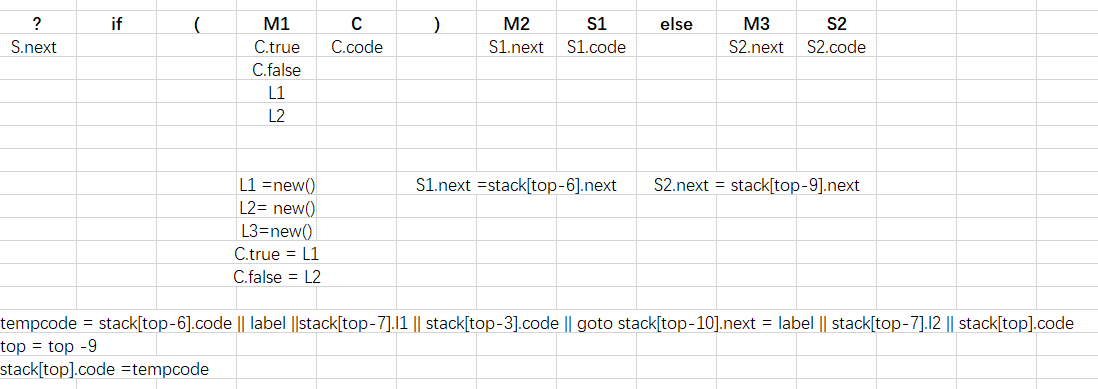
\includegraphics[scale=0.6]{chapter5_hw3_4}
\end{figure}

\begin{figure}[H]
\centering
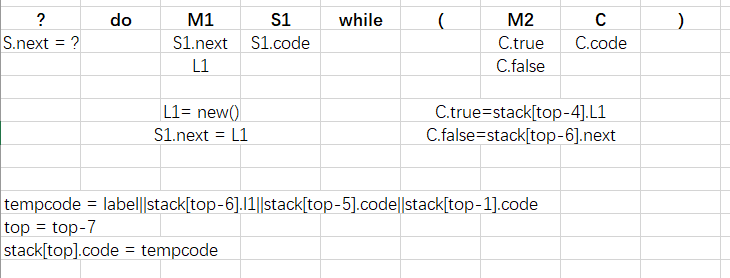
\includegraphics[scale=0.6]{chapter5_hw3_5}
\end{figure}

\begin{figure}[H]
\centering
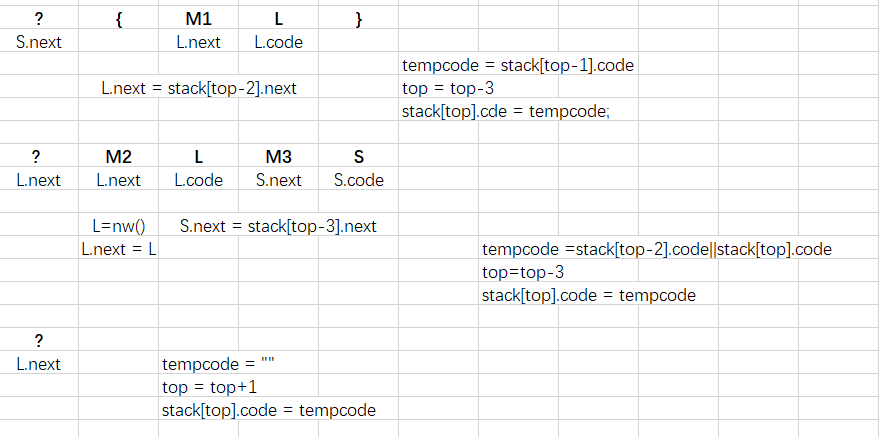
\includegraphics[scale=0.6]{chapter5_hw3_6}
\end{figure}


\end{document}
